\documentclass[11pt]{article}
\usepackage[utf8]{inputenc} % Para caracteres en español
\usepackage{amsmath,amsthm,amsfonts,amssymb,amscd}
\usepackage{multirow,booktabs}
\usepackage[table]{xcolor}
\usepackage{fullpage}
\usepackage{tikz}
\usepackage{physics}

%%
\usepackage{pgfplots}
\usepgfplotslibrary{polar}
\usepgflibrary{shapes.geometric}
\usetikzlibrary{calc}


\pgfplotsset{my style/.append style={axis x line=middle, axis y line=
           middle, xlabel={$x$}, ylabel={$y$}, axis equal }}
\pgfplotsset{my style-2/.append style={axis x line=middle, axis y line=
           middle, xlabel={$x$}, ylabel={$y$}}}


\usetikzlibrary{arrows, circuits.ee.IEC, positioning}
\usepackage[american voltages, american currents,siunitx]{circuitikz}

\usepackage{lastpage}
\usepackage{enumitem}
\usepackage{fancyhdr}
\usepackage{mathrsfs}
\usepackage{wrapfig}
\usepackage{setspace}
\usepackage{calc}
\usepackage{multicol}
\usepackage{cancel}
\usepackage[retainorgcmds]{IEEEtrantools}
\usepackage[margin=3cm]{geometry}
\usepackage{amsmath}
\newlength{\tabcont}
\setlength{\parindent}{0.0in}
\setlength{\parskip}{0.05in}
\usepackage{empheq}
\usepackage{framed}
\usepackage[most]{tcolorbox}
\usepackage{xcolor}
\colorlet{shadecolor}{orange!15}
\parindent 0in
\parskip 12pt
\geometry{margin=1in, headsep=0.25in}
\theoremstyle{definition}
\newtheorem{defn}{Definition}
\newtheorem{reg}{Rule}
\newtheorem{exer}{Exercise}
\newtheorem{note}{Note}
\usepackage[english]{babel}
\usepackage[protrusion=true,expansion=true]{microtype}  
\usepackage{amsmath,amsfonts,amsthm,amssymb}
\usepackage{graphicx}
\usepackage{tcolorbox}
\usepackage{amssymb}
\tcbuselibrary{theorems}
\newtcbtheorem
  []% init options
  {definition}% name
  {Definition}% title
  {%
    colback=green!5,
    colframe=green!35!black,
    fonttitle=\bfseries,
  }% options
  {def}% prefix

\newtcbtheorem
  []% init options
  {lemma}% name
  {Lemma}% title
  {%
    colback=yellow!5,
    colframe=orange!110,
    fonttitle=\bfseries,
  }% options
  {lem}% prefix

\newtcbtheorem
  []% init options
  {theorem}% name
  {Theorem}% title
  {%
    colback=yellow!5,
    colframe=orange!110,
    fonttitle=\bfseries,
  }% options
  {thm}% prefix

\newtcbtheorem
  []% init options
  {solution}% name
  {Solution}% title
  {%
    colback=magenta!5,
    colframe=magenta!150,
    fonttitle=\bfseries,
  }% options
  {not}% prefix

\newtcbtheorem
  []% init options
  {example}% name
  {Example}% title
  {%
    colback=red!5,
    colframe=red!100,
    fonttitle=\bfseries,
  }% options
  {exm}% prefix


\newtcbtheorem
  []% init options
  {algorithm}% name
  {Algorithm} %title
  {%
    colback=blue!5,
    colframe=blue!100,
    fonttitle=\bfseries,
  }% options
  {alg}% prefix

\newtcbtheorem
  []% init options
  {properties}% name
  {Properties}% title
  {%
    colback=green!5,
    colframe=green!35!black,
    fonttitle=\bfseries,
  }% options
  {pro}% prefix



% Sets
\newcommand{\N}{\ensuremath{\mathbb{N}}}
\newcommand{\Z}{\ensuremath{\mathbb{Z}}}
\newcommand{\Q}{\ensuremath{\mathbb{Q}}}
\newcommand{\R}{\ensuremath{\mathbb{R}}}
\newcommand{\C}{\ensuremath{\mathbb{C}}}
\newcommand{\F}{\ensuremath{\mathbb{F}}}
\newcommand{\Mnn}{\ensuremath{M_{n \times n}}}
\newcommand{\sym}{\mathbin{\triangle}}
\newcommand{\stcomp}[1]{{#1}^\complement}

% Operators
\newcommand{\Rarr}{\Rightarrow}
\newcommand{\Larr}{\Leftarrow}
\newcommand{\Harr}{\Leftrightarrow}
\newcommand{\harr}{\leftrightarrow}
\newcommand{\dyx}{\dv{y}{x}}

% Linear Algebra
\newcommand{\vui}{\mathbf{\hat{\textnormal{\bfseries\i}}}}
\newcommand{\vuj}{\mathbf{\hat{\textnormal{\bfseries\j}}}}
\newcommand{\xto}{\xrightarrow} % \xto{R_1 \harr R_2}
\newcommand{\cbm}[2]{\ensuremath{{}_{#1}[I]{}_{#2}}} % change of basis matrix
\DeclareMathOperator{\Proj}{Proj}
\DeclareMathOperator{\Perp}{Perp}
\DeclareMathOperator{\Span}{Span}
\DeclareMathOperator{\Col}{Col}
\DeclareMathOperator{\adj}{adj}

\newcommand{\QType}{Q}
\newcounter{question}[subsection]
\renewcommand{\thequestion}{\QType\ifnum\value{question}<10 0\fi\arabic{question}}
\newcommand{\question}{\par\refstepcounter{question}\textbf{\thequestion}.\space}

\renewcommand\qedsymbol{$\blacksquare$}



\title{Applications of Linear Algebra}
\author{Abdullah Zubair}
\date{\today}

\begin{document}

\maketitle

This paper will explore the applications of linear algebra, an interesting yet elegant field of applied mathematics. The applications themselves may be rather trivial to most readers, however the intent is to demonstrate how such applications may be solved, or approached more efficiently using linear algebra. 

\section{Circuit Applications}
Let us consider the following circuit where the current flow through each load is unknown.


\begin{center}

\begin{comment}

\begin{circuitikz}[x=1.5cm,y=1.5cm]
\ctikzset{label/align=smart,bipoles/length=1.5cm}
\draw (0,0) to[R,l_=\mbox{$R_1=\SI{2}{\ohm}$},*-*] (4,0);
\draw (2,3) to[R,l^=\mbox{$R_2=\SI{2}{\ohm}$},*-*] (4,0);
\draw (0,0) to[R,l_=\mbox{$R_3=\SI{2}{\ohm}$},*-*] (2,3);
\end{circuitikz}

\end{comment}

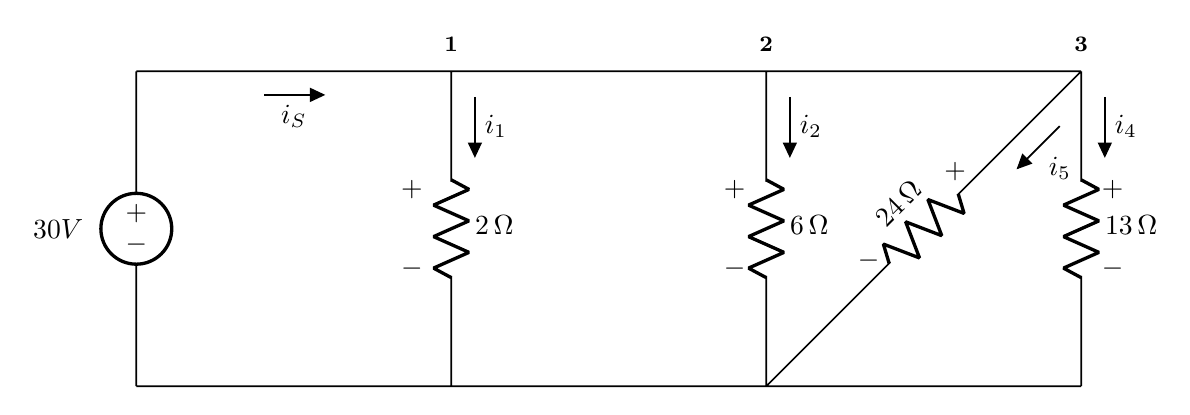
\begin{tikzpicture}[circuit ee IEC,american voltages,x=2cm,y=2cm, semithick, every info/.style={font=\footnotesize}, small circuit symbols, set resistor graphic=var resistor IEC graphic]
\ctikzset{label/align=smart,bipoles/length=1.5cm}
     \draw (0,0) -- (6,0)
    (0,2) to [V, v_=\mbox{$30 V$}] (0,0)
    (1.75,1.25) node{$+$}
    (1.75,0.75) node{$-$}
    (2,2) node[label={[font=\footnotesize]above:\textbf{1}}] {}
    (0,2) to [short, f_=$i_S$]  (2,2)
    (2,2) -- (4,2)
    (2,2) to [short, f=$i_1$] (2,1.3)
    (4,2) node[label={[font=\footnotesize]above:\textbf{2}}] {}
    (2,2) to [R, l=\mbox{$\SI{2}{\ohm}$}] (2,0)
    (4,2) to [short, f=$i_2$] (4,1.3)
    (3.8,1.25) node{$+$}
    (3.8,0.75) node{$-$}
    (4,2) -- (6,2)
    (4,2) to [R, l=\mbox{$\SI{6}{\ohm}$}] (4,0)
    (6,2) to [R, l=\mbox{$\SI{13}{\ohm}$}] (6,0)
    (4,0) to [R, l=\mbox{$\SI{24}{\ohm}$}] (6,2)
    (6,2) to [short, f=$i_4$,] (6,1.3)
    (6,2) to [short, f=$i_5$,] (5.25,1.25)
    (5.2,1.36) node{$+$}
    (4.65,0.8) node{$-$}
    (6,2) node[label={[font=\footnotesize]above:\textbf{3}}] {}
    %(5,2) to [short, f_=$i_4$, *-*] (5,1.2)
    (6.2, 1.25) node{$+$}
    (6.2, 0.75) node{$-$};


\end{tikzpicture}
\end{center}



We proceed by applying Kirchoffs current/voltage laws to deduce a set of equations from which we can construct a matrix and reduce to RREF to obtain a solution to the unknown current values. To make our solution slightly more concise we will make use of a well known circuit technique whereby we treat the three nodes denoted in the circuit as a single node and proceed as follows,

\begin{center}
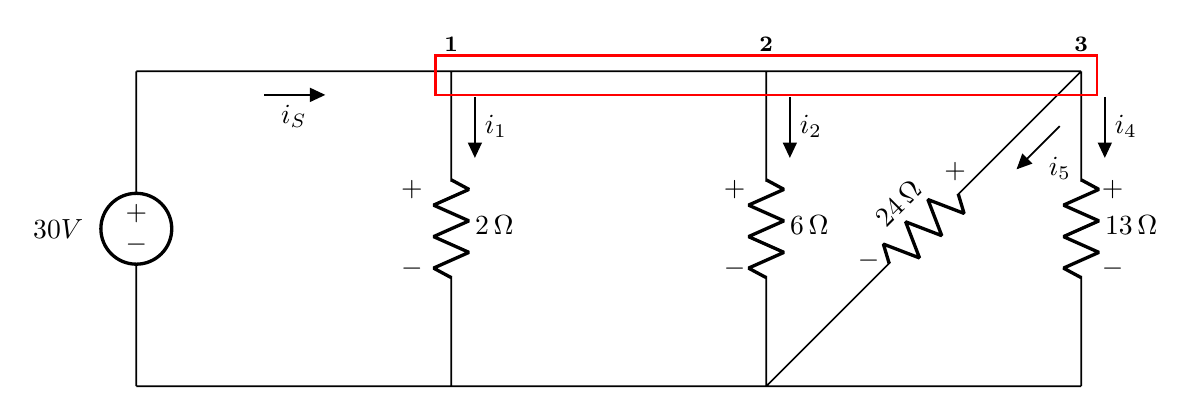
\begin{tikzpicture}[circuit ee IEC,american voltages,x=2cm,y=2cm, semithick, every info/.style={font=\footnotesize}, small circuit symbols, set resistor graphic=var resistor IEC graphic]
\ctikzset{label/align=smart,bipoles/length=1.5cm}
     \draw (0,0) -- (6,0)
    (0,2) to [V, v_=\mbox{$30 V$}] (0,0)
    (1.75,1.25) node{$+$}
    (1.75,0.75) node{$-$}
    (2,2) node[label={[font=\footnotesize]above:\textbf{1}}] {}
    (0,2) to [short, f_=$i_S$]  (2,2)
    (2,2) -- (4,2)
    (2,2) to [short, f=$i_1$] (2,1.3)
    (4,2) node[label={[font=\footnotesize]above:\textbf{2}}] {}
    (2,2) to [R, l=\mbox{$\SI{2}{\ohm}$}] (2,0)
    (4,2) to [short, f=$i_2$] (4,1.3)
    (3.8,1.25) node{$+$}
    (3.8,0.75) node{$-$}
    (4,2) -- (6,2)
    (4,2) to [R, l=\mbox{$\SI{6}{\ohm}$}] (4,0)
    (6,2) to [R, l=\mbox{$\SI{13}{\ohm}$}] (6,0)
    (4,0) to [R, l=\mbox{$\SI{24}{\ohm}$}] (6,2)
    (6,2) to [short, f=$i_4$,] (6,1.3)
    (6,2) to [short, f=$i_5$,] (5.25,1.25)
    (5.2,1.36) node{$+$}
    (4.65,0.8) node{$-$}
    (6,2) node[label={[font=\footnotesize]above:\textbf{3}}] {}
    %(5,2) to [short, f_=$i_4$, *-*] (5,1.2)
    (6.2, 1.25) node{$+$}
    (6.2, 0.75) node{$-$};
    \draw[red, thick] (1.9,2.1) rectangle (6.1,1.85);


\end{tikzpicture}
\end{center}


\end{document}

